\subsubsection{Frontend Architecture and Implementation}
In the development of this project, we adopted a modern web development stack that incorporated a combination of cutting{-}edge technologies aimed at optimizing performance, scalability, and maintainability. The integration of these technologies facilitated the creation of a highly efficient and user{-}friendly web application. This section provides a comprehensive overview of the key technologies used in the frontend of the application, outlining their individual roles and how they collectively contributed to the success of the project.
\begin{enumerate}
    \item{} \textbf{React}

     React is a widely used and powerful JavaScript/TypeScript library that is primarily designed for building user interfaces. It was chosen for this project due to its ability to facilitate the development of dynamic and responsive web applications. In conjunction with \textbf{Next.js}, React allowed for the implementation of a component{-}driven architecture. This architectural approach enables the reuse of individual UI components throughout the application, which not only streamlined the development process but also ensured greater maintainability in the long term. By breaking down the user interface into smaller, reusable components, we were able to manage and scale the application more effectively. React’s virtual DOM mechanism also ensured efficient rendering of changes to the UI, contributing to an enhanced user experience by minimizing the amount of time required to update the interface.
     
    Moreover, React’s active community and vast ecosystem of libraries and tools made it easier to integrate other technologies and features into the application, further improving its overall functionality and performance. As a result, React played a crucial role in enabling a seamless, interactive experience for users, while also enhancing the maintainability and scalability of the codebase.

    \item{} \textbf{Next.js}
    
    Next.js is a robust React framework that extends the capabilities of React by offering features such as server{-}side rendering (SSR) and static site generation (SSG). These features proved to be essential for optimizing the application's load times, which was critical to the project’s success. Server{-}side rendering allows the server to generate the HTML for the page on each request, as opposed to client{-}side rendering where the browser must first download and execute JavaScript to generate the page. This process significantly reduces the time required for the page to be displayed to the user, resulting in a faster and more efficient application.

    Additionally, Next.js’ static site generation capabilities allowed us to pre{-}render pages at build time, meaning that the application could serve static HTML files for commonly accessed pages, further enhancing performance. The combination of SSR and SSG enabled a smooth and responsive user experience.

    Next.js also provided a robust routing system that made it easier to manage the application’s navigation. The framework’s file{-}based routing system allowed for simple, declarative routing, which contributed to the overall maintainability of the project. Next.js’ out{-}of{-}the{-}box support for features like code splitting and automatic optimization ensured that the application remained highly performant, even as it grew in complexity.


    \item{} \textbf{TailwindCSS}

    For styling the application, \textbf{TailwindCSS}, a utility{-}first CSS framework, was chosen for its ability to enable rapid UI development. Unlike traditional CSS frameworks, which rely on pre{-}defined UI components and styles, TailwindCSS provides low{-}level utility classes that can be combined to build custom designs. This approach allowed for greater flexibility in styling the application, as developers were able to apply precise and granular control over the UI without the need for writing custom CSS from scratch.

    One of the key advantages of using TailwindCSS was the speed with which we could implement and modify styles. By utilizing utility classes, we were able to quickly experiment with different design configurations and make adjustments on the fly. This approach also minimized the need for additional CSS files, reducing the overall complexity of the styling process.

    In addition to TailwindCSS, we incorporated several tools to enhance the framework’s capabilities. \textbf{Tailwind{-}merge} was used to intelligently combine conflicting utility classes, ensuring that styles were applied consistently throughout the application. \textbf{TailwindCSS{-}animate} provided utility classes for adding animations, which helped bring dynamic visual elements to life without needing to write custom animation logic. These tools, when used in tandem, allowed for more advanced styling and complex animations while maintaining the simplicity and ease of use that TailwindCSS is known for.

    \item{} \textbf{Mapbox GL and React Map GL} \\
    The integration of interactive maps and advanced visualization features played a key role in the functionality of the project. For this purpose, we utilized \textbf{Mapbox GL} and \textbf{React Map GL}. \textbf{Mapbox GL} is a powerful mapping library that provides advanced capabilities for rendering interactive maps with smooth transitions and animations. It is built to handle large datasets, enabling the display of dynamic geospatial information with high performance and precision. Mapbox GL was used to power the core mapping functionality of the application, allowing users to interact with maps seamlessly.

    To integrate Mapbox GL with our React application, we used \textbf{React Map GL}, a library that provides a simple wrapper around Mapbox GL, making it easier to embed and control interactive maps within React components. React Map GL allowed us to leverage the full potential of Mapbox GL while maintaining a consistent and efficient React{-}based architecture.

    In addition to basic mapping functionality, we integrated \textbf{Deck.gl} for advanced data visualization. Deck.gl is a framework that enhances Mapbox GL by enabling the display of complex data visualizations on top of interactive maps. This was particularly beneficial for our project, as it allowed us to visualize large datasets in an efficient and interactive manner, providing users with a rich and engaging experience.

    \item{} \textbf{ShadCN/UI} \\
    To streamline the development of UI components, we incorporated \textbf{ShadCN}, a component library built on top of \textbf{Radix Primitives}. ShadCN combines the flexibility of Radix UI with a more opinionated design system, tailored for projects that require custom styling with the power of TailwindCSS\@. Radix Primitives offers a set of low{-}level UI components that are highly customizable, accessible, and composable, making them ideal for building complex user interfaces.

    By using ShadCN, we were able to access a suite of pre{-}built, customizable components that adhered to accessibility standards, ensuring that our application was usable by all users, including those with disabilities. ShadCN's integration with Radix Primitives allowed us to quickly implement accessible and customizable components, reducing the need for additional development and ensuring consistency across the application.

    The combination of ShadCN’s flexible components and TailwindCSS allowed us to build a visually appealing and highly functional user interface with minimal configuration. Furthermore, ShadCN's tight integration with accessibility guidelines ensured that the application met the required standards for usability, providing an inclusive experience for all users.

    \item{} \textbf{Radix Primitives} \\
    Radix Primitives played a crucial role in the design and development of our user interface components. Radix Primitives provides a set of foundational, high{-}quality UI components that serve as the core building blocks for any application. These components are unstyled and highly customizable, giving developers full control over the look and behaviour of the elements while ensuring accessibility and functionality out of the box.

    The core of Radix Primitives includes essential UI elements such as buttons, modals, popovers, sliders, tabs, and other interactive components. These primitives are designed to be flexible and composable, allowing developers to combine them in various ways to create complex UI patterns. The components are built to be accessible, ensuring that the user interface remains usable for all users, including those with disabilities, without requiring additional development effort to meet accessibility standards.

    One of the standout features of Radix Primitives is its focus on accessibility. The components are designed with built{-}in features like keyboard navigation, screen reader support, and proper focus management. This allows the application to be fully functional and accessible across a wide range of devices and assistive technologies, without the need for custom implementation of these features. As accessibility is a fundamental aspect of modern web development, Radix Primitives ensured that the project adhered to the highest standards for inclusive design.

    In addition to accessibility, Radix Primitives allows for extensive customization. While the components come with sensible defaults, they are unstyled, which provides the flexibility to apply custom styles that match the overall design language of the application. This level of customization allowed the development team to ensure that the UI components blended seamlessly with the rest of the application’s design. By combining Radix Primitives with **TailwindCSS**, we could easily customize the components using utility{-}first CSS classes, speeding up the styling process and ensuring consistency across the entire application.

    The composability of Radix Primitives also played a significant role in the project's development. The library is designed to allow developers to create complex user interface patterns by combining simple components in flexible ways. For instance, we could easily integrate modal dialogs, dropdown menus, and tooltips to form cohesive UI patterns that enhanced the user experience. This approach not only saved development time but also reduced the likelihood of introducing bugs, as we could rely on well{-}tested, standardized components rather than building these features from scratch.

    By leveraging Radix Primitives, we were able to focus on creating a polished and accessible user interface while avoiding the complexity of building low{-}level components. The ability to use these pre{-}built, flexible primitives allowed us to deliver a high{-}quality user experience with minimal overhead. Radix Primitives was an essential tool in ensuring that the application was both user{-}friendly and accessible, all while maintaining the flexibility to customize and extend the components as needed for the project.


\end{enumerate}

The integration of these technologies into the frontend of the project provided a solid foundation for building a high{-}performance, scalable, and user{-}friendly web application. From the server{-}side rendering capabilities of Next.js to the highly customizable components offered by ShadCN, each technology played a critical role in the overall success of the project. The use of React and Next.js allowed for a modular and efficient development process, while TailwindCSS and its associated tools streamlined the styling process and enabled rapid UI development. The incorporation of Mapbox GL and Deck.gl brought advanced mapping and data visualization capabilities to the application, making it more interactive and engaging for users. Together, these technologies enabled us to deliver an application that met high standards of code quality, user experience, and performance, ensuring its success in achieving the project’s objectives.

\subsubsection{Client State Management}
    \paragraph{Introduction}\mbox{}

    Effective client state management is a crucial aspect of the \textbf{Magpie} frontend, as it ensures a seamless and consistent user experience. Given the dynamic nature of the application, with interactive elements such as maps, search filters, and property details, it is essential to maintain synchronization between different UI components while preventing errors and inconsistencies. Managing state efficiently is particularly important when handling large datasets that need to be presented in a user{-}friendly manner across various parts of the application.
    \paragraph{React Context}\mbox{}

    To achieve this, the application employs state management techniques that allow for centralized control of the application’s state. One of the core tools used for this purpose is \textbf{React Context}, which provides a simple way to share state across multiple components without having to pass data manually through props. React Context enables the application to manage the user’s preferences, search filters, and saved properties in a global state, ensuring that these settings are accessible across various parts of the application. This method of state management is particularly useful for dynamic features, such as filtering search results based on user input or retaining user selections when navigating between different pages or sections of the platform.
    \paragraph{Redux}\mbox{}

    In addition to React Context, the use of more advanced state management libraries such as Redux can be considered for larger{-}scale applications that require more complex state handling. Redux facilitates a unidirectional data flow and provides a centralized store that allows the state to be updated in a predictable manner. With Redux, the application can ensure that all components are working with the most up{-}to{-}date information, whether that involves real{-}time data from maps or user{-}selected property preferences. Redux also allows for more complex actions, such as asynchronous data fetching, and can be used in conjunction with middleware like Redux Thunk for handling side effects, further enhancing the application’s performance and stability.
    \paragraph{Consistent User Experience}\mbox{}

    Client state management also ensures that the data displayed to the user remains consistent. For instance, when a user interacts with a map, the system must track the map's current state and the filter options that the user has selected. By maintaining this state across different components, users can switch between different views (such as property details and map views) without losing their previous selections. Additionally, state management ensures that updates to the user interface, such as property filtering or adding a property to the favourites list, are reflected across the entire application in real{-}time, maintaining data integrity and providing users with a smooth browsing experience.
    \paragraph{Conclusion}\mbox{}

    Overall, client state management plays a vital role in improving the usability and responsiveness of the frontend, reducing redundancy and complexity by centralizing control over the application’s data. This centralized management allows for easier maintenance and scalability as the application evolves and new features are added.

\subsubsection{UI Walkthrough}
\begin{figure}[h]
    \centering{}
    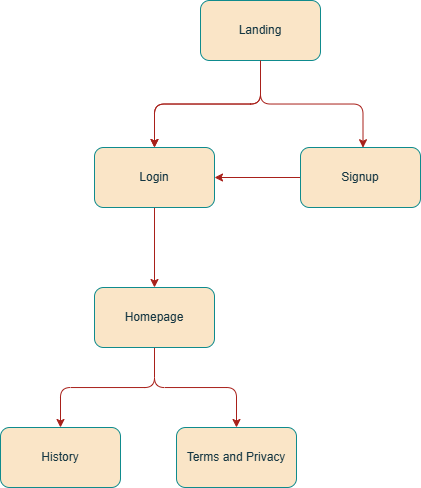
\includegraphics[width=0.6\textwidth]{images/site/sitemap.png}
    \caption{Site map {-} magpie}
\end{figure}
\paragraph{Landing Page}\mbox{}\\
\textbf{Introduction}

Upon accessing the landing page, users are greeted with a clean and modern layout that introduces them to `Magpie' {-} a geographical information service providing a glance at available public services in Dublin. The layout is designed to be visually appealing, with prominent calls to action and easily navigable sections.

\textbf{Header Section}

\begin{figure}[h]
    \centering{}
    
\includegraphics[width=1\textwidth]{images/site/landing/landing_6_header.png}
    \caption{Landing page {-} Header}
\end{figure}
\begin{itemize}
    \item{} \textbf{Navigation Bar:} At the top of the page, the navigation bar features the \textbf{Magpie logo} on the left side, offering a simple and recognizable brand identity. To the right, navigation links for \textbf{About}, \textbf{Features}, \textbf{Use Cases}, and \textbf{Get Started} provide quick access to key sections. Additionally, a \textbf{Sign Up} button stands out in black with white text for clear calls to action.
    \item{} \textbf{Mobile Menu:} For mobile views, a hamburger menu (three horizontal lines) appears, ensuring that the navigation remains compact and accessible on smaller screens.
\end{itemize}

\textbf{Hero Section}

\begin{figure}[h]
    \centering{}
    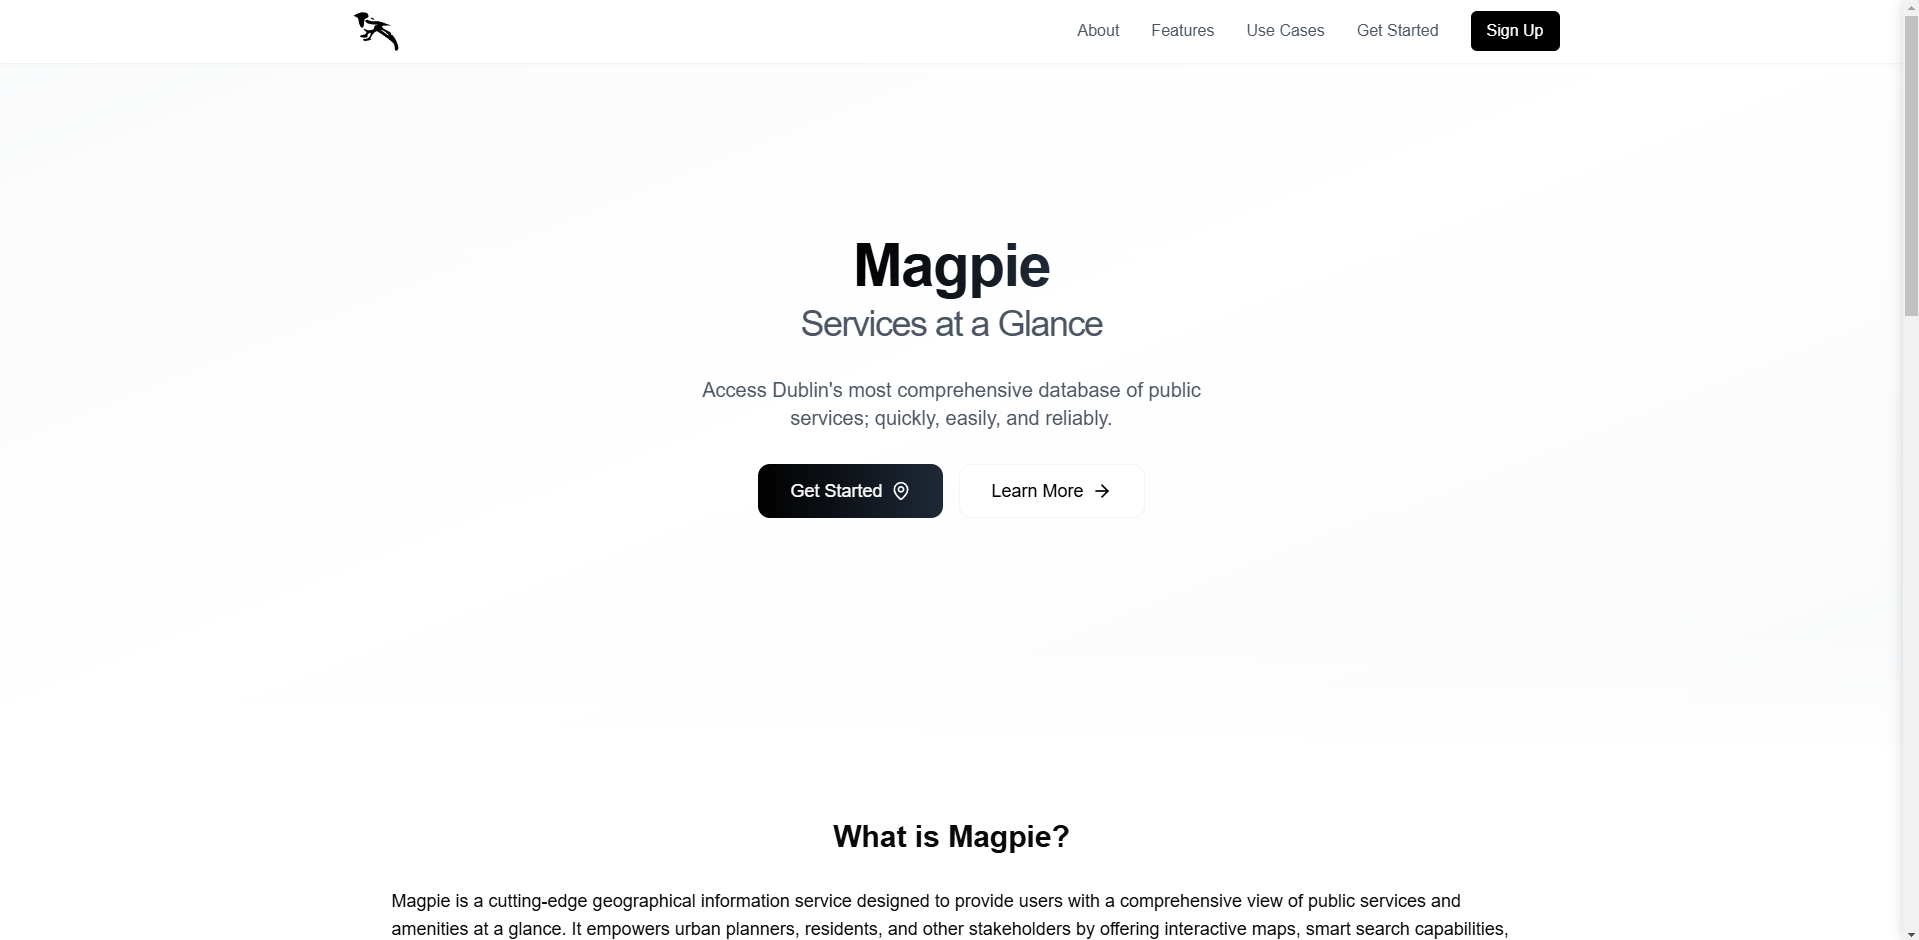
\includegraphics[width=1\textwidth]{images/site/landing/landing_1_hero.png}
    \caption{Landing page {-} Hero section}
\end{figure}

\begin{itemize}
    \item{} \textbf{Headline:} The page features a bold, eye{-}catching headline that reads `Magpie' in a gradient text style, followed by the tagline `Services at a Glance.' This is a clear and engaging introduction to the site's purpose.
    \item{} \textbf{Subheading:} A short description reinforces the value proposition: `Access Dublin's most comprehensive database of public services; quickly, easily, and reliably.' This emphasizes the platform's utility and target audience.
    \item{} \textbf{Primary CTA:} A large button titled `Get Started' invites users to sign up or log in, accompanied by an icon of a map pin to add a visual cue to the call to action.
    \item{} \textbf{Secondary CTA:} A `Learn More' button encourages users to explore more details about the platform. It’s designed to stand out but with a lighter visual treatment compared to the primary CTA\@.
\end{itemize}

\newpage{}

\textbf{About Section}

\begin{figure}[h]
    \centering{}
    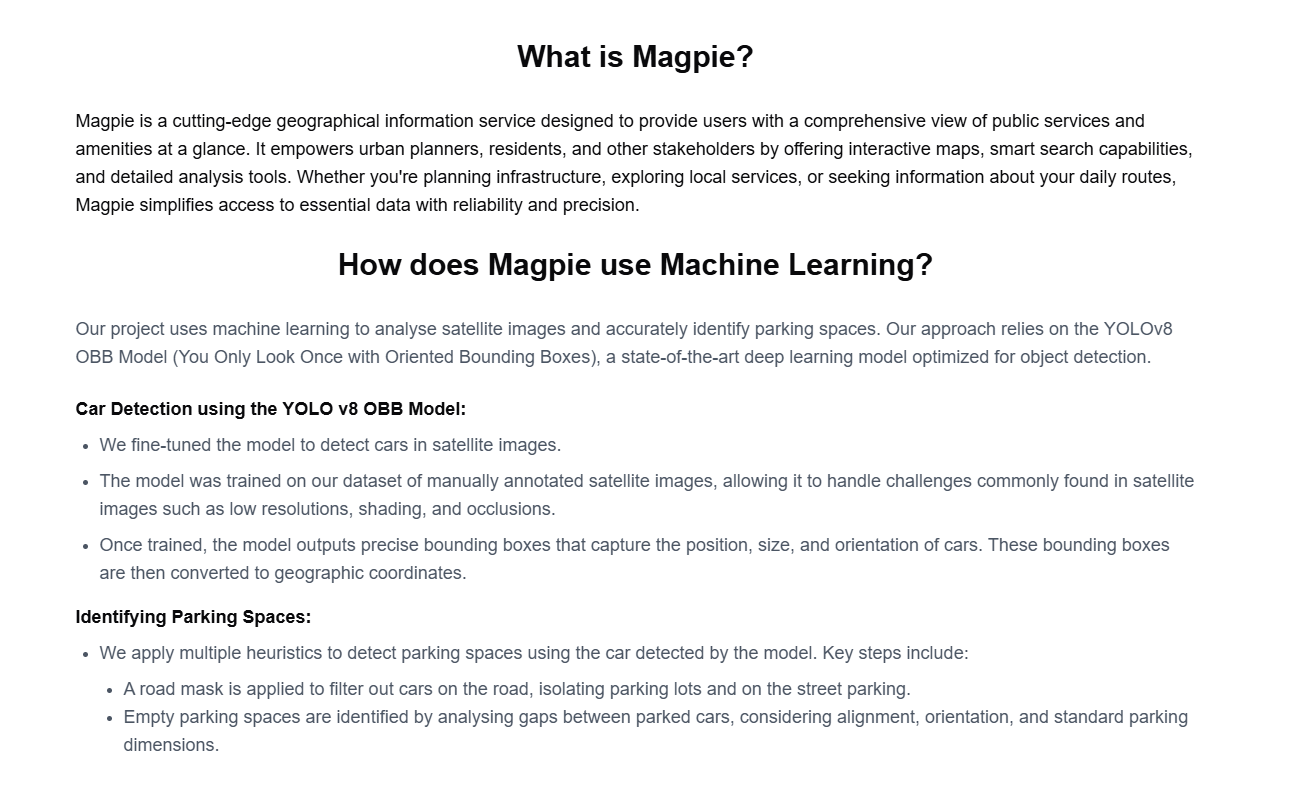
\includegraphics[width=1\textwidth]{images/site/landing/landing_2_about.png}
    \caption{Landing page {-} About section}
\end{figure}

\textbf{What is Magpie?:} This section introduces \textbf{Magpie} as a \textbf{geographical information service}, explaining its functionality and target users. It emphasizes its usefulness for urban planners, residents, and other stakeholders by providing interactive maps, smart search capabilities, and detailed analysis tools.

\textbf{How Magpie Uses Machine Learning:} This section explains the use of \textbf{machine learning} to analyze satellite images and detect parking spaces. It provides insight into the model used (YOLOv8 OBB), detailing how it detects cars and identifies available parking spaces. A breakdown of the process offers technical depth while remaining accessible to a general audience.

\textbf{Features Section}

\begin{figure}[h]
    \centering{}
    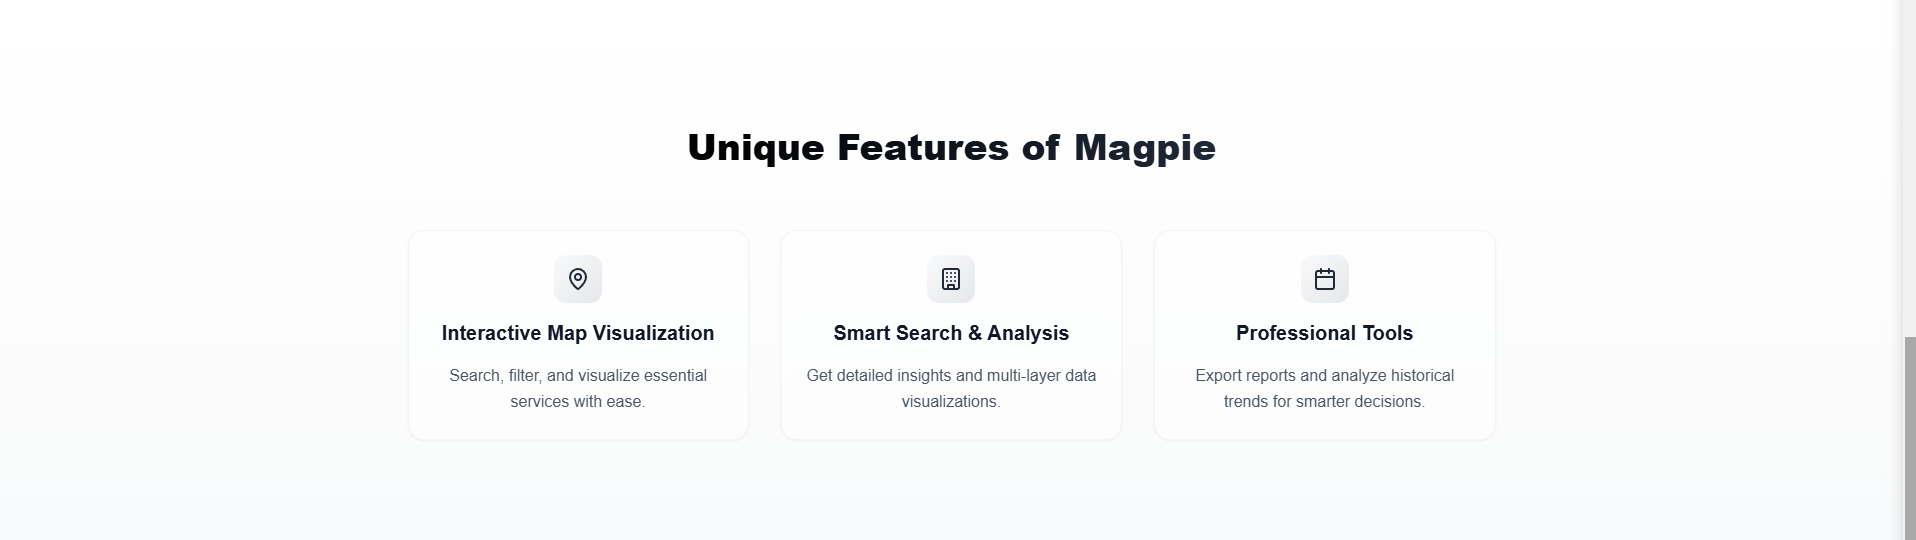
\includegraphics[width=1\textwidth]{images/site/landing/landing_3_features.png}
    \caption{Landing page {-} Features section}
\end{figure}

\textbf{Unique Features {-} } This section highlights the core capabilities of Magpie:

\begin{itemize}
    \item{} \textbf{Interactive Map Visualization:} The ability to search, filter, and visualize services through an interactive map.
    \item{} \textbf{Smart Search \& Analysis:} Provides detailed insights with multi{-}layer data visualizations.
    \item{} \textbf{Professional Tools:} Features designed to export reports and analyze historical trends.
\end{itemize}

Each feature is represented by a card that contains an icon, a title, and a brief description. Hovering over these cards gives users more details, encouraging them to explore further.


\textbf{Use Case section}

\begin{figure}[h]
    \centering{}
    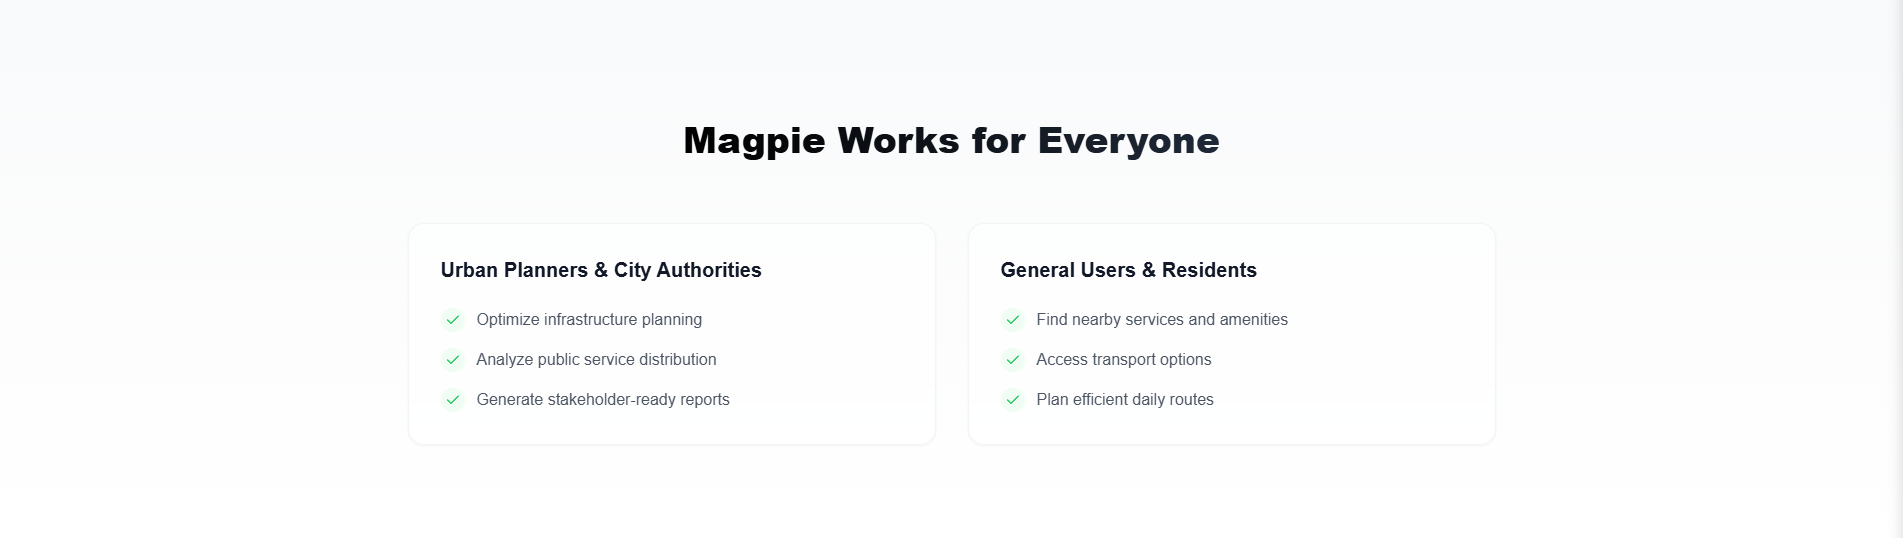
\includegraphics[width=1\textwidth]{images/site/landing/landing_4_usecases.png}
    \caption{Landing page {-} Use Case section}
\end{figure}

\textbf{Magpie Works for Everyone:} This section presents specific use cases for different user types:
\begin{itemize}
    \item{}  \textbf{Urban Planners \& City Authorities:} Features such as optimizing infrastructure, analysing service distribution, and generating reports.
    \item{} \textbf{General Users \& Residents:} Services to find nearby amenities, access transport options, and plan efficient routes.
\end{itemize}

\textbf{Call To Action (CTA) Section}

\begin{figure}[h]
    \centering{}
    
\includegraphics[width=1\textwidth]{images/site/landing/landing_5_cta.png}
    \caption{Landing page {-} CTA section}
\end{figure}

\begin{itemize}
    \item{} \textbf{Ready to Transform How You Plan?:} The page concludes with a strong call to action, urging users to \textbf{sign up} and start using Magpie. This section reiterates the platform's value in making data{-}driven decisions, featuring a large, attention{-}grabbing button labelled `Sign Up Now.'
    \item{} \textbf{Gradient Background:} The footer section features a subtle gradient background, reinforcing the design's sleek and modern aesthetic.
\end{itemize}

The landing page for \textbf{Magpie} is designed to effectively introduce the platform’s features, functionality, and benefits through a series of engaging sections. The page focuses on presenting Magpie as a user{-}friendly tool for urban planners and residents, with clear calls to action and visually appealing design elements. It balances technical information with an approachable layout, ensuring that both potential users and technical stakeholders can easily understand its offerings.

\newpage{}

\textbf{Signup Page}

\begin{figure}[h]
    \centering{}
    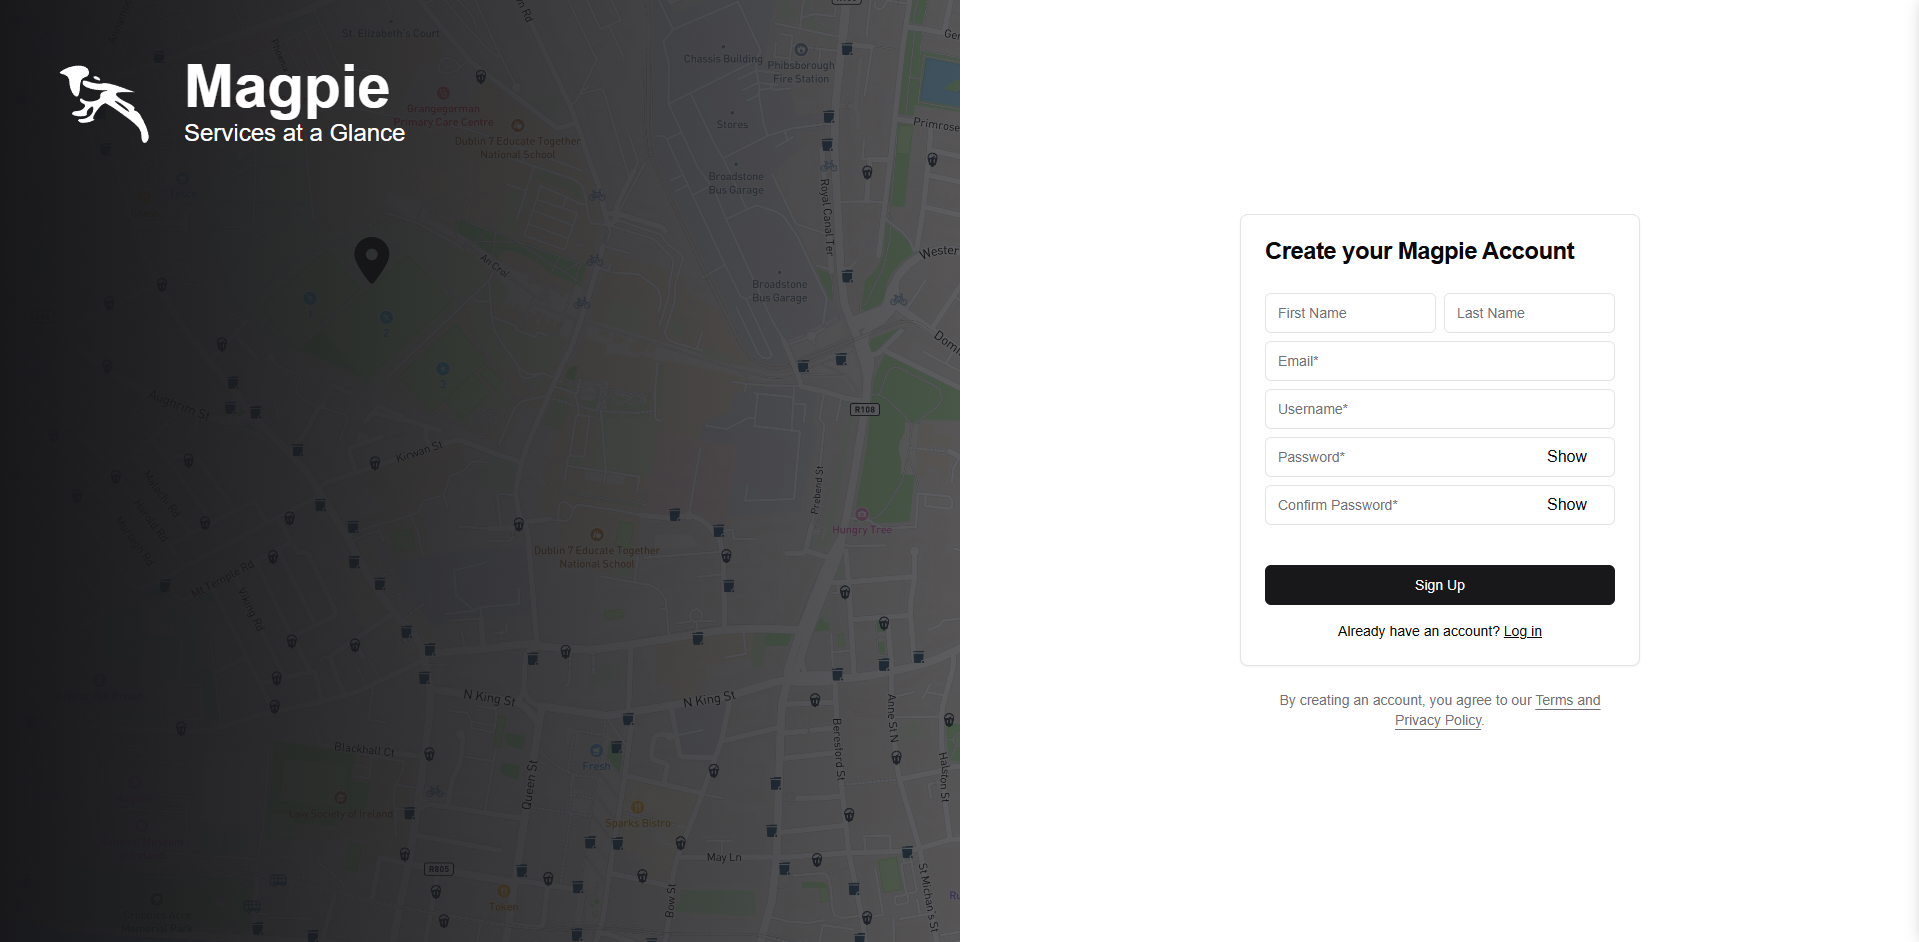
\includegraphics[width=1\textwidth]{images/site/signup/signup_page.png}
    \caption{The Signup Page}
\end{figure}

The \textbf{Signup} page serves as the gateway for users to create an account on Magpie. It is designed with a straightforward layout to guide users through the process of entering their personal information securely.

\textbf{Header Section}

The header section plays a crucial role in establishing the identity of the page.
\begin{itemize}
    \item{} \textbf{Magpie Logo:} Positioned prominently at the top of the page is the \textbf{Magpie logo}, providing immediate brand recognition. The logo’s size and placement are intentional to make it easy for users to identify the platform and navigate back to the homepage, should they need to.
    \item{} \textbf{Tagline:} Below the logo, the tagline \textbf{`Services at a Glance'} emphasizes the platform's purpose, providing a succinct description of its functionality{-}offering users quick access to available public services in Dublin.
    \item{} \textbf{Call to Action:} The headline in the header invites users to \textbf{Create your Magpie Account} in large, bold text, making the goal of the page clear and guiding users toward account creation. This is an important call to action that users are encouraged to follow.
\end{itemize}

\textbf{Form Inputs}

The heart of the Signup page is the \textbf{form inputs}, where users input their details to create an account.

\begin{itemize}
    \item{} \textbf{Required Fields:}
    \begin{itemize}
        \item{} \textbf{First Name} and \textbf{Last Name} fields ensure that the platform has accurate personal information about the user. These fields are essential for building a profile that can be used for various personalization features across the Magpie platform. 
        \item{} \textbf{Email Address} is also required, which is important for account verification, password recovery, and communication with the platform. Users are reminded that this email will be used for correspondence related to their account.
        \item{} \textbf{Username} allows the user to choose a unique identifier for logging into the platform. This is an important step in personalizing the account, as the username will be used alongside the password to access the Magpie dashboard. 
    \end{itemize}
    \item{} \textbf{Password Fields:}
    \begin{itemize}
        \item{} The \textbf{Password} field is critical for securing the account, and users are encouraged to choose a strong, secure password.
        \item{} A \textbf{Confirm Password} field is included for verification to reduce errors and ensure that users input their password correctly.
        \item{} \textbf{Password Visibility Toggle:} A key feature for convenience is the \textbf{toggle} to show or hide the password as users type. This helps users ensure they’ve entered the correct password without exposing it to others around them.
    \end{itemize}
\end{itemize}

\textbf{Call To Action}

\begin{itemize}
    \item{}  \textbf{Sign Up Button:} The page features a prominent \textbf{Sign Up} button in the center of the form. The button is large and visually distinct to stand out, ensuring that users know where to click to complete their registration once all fields are filled. The button uses an eye{-}catching color, making it easy to find.
    \item{} \textbf{Link to Log In:} A secondary, less prominent link underneath the main form invites users who already have an account to \textbf{Log in}. This ensures that returning users do not feel lost and can quickly find their way to the login page.
\end{itemize}

\textbf{Terms and Privacy}

\begin{itemize}
    \item{} \textbf{Consent to Terms:} At the bottom of the form, there is an important reminder for users that by signing up for the platform, they agree to Magpie's \textbf{Terms and Privacy Policy}. This ensures that users are informed about the platform’s legal agreements before proceeding. 
    \item{} \textbf{Link to Terms:} A clickable link is provided for users to read the \textbf{Terms and Privacy Policy} in detail. The link opens the full document, so users have access to the complete legal information regarding their data, privacy, and the platform's use.
\end{itemize}

\textbf{Overall Design and Experience}

The design of the signup page is intuitive and responsive, providing a smooth experience for users on both desktop and mobile devices. It is minimalistic, focusing on the essential information without distractions, while the color scheme and layout are optimized for clarity and usability. The goal of the page is to simplify the signup process, ensuring that users can easily create their accounts while being informed about the necessary legal terms.

This page ensures that users feel confident about creating an account by making the process as straightforward as possible while providing clear information about data privacy and platform policies. The inclusion of visual cues like the password visibility toggle and clearly marked sections for each field enhances usability, contributing to a positive user experience.



\newpage{}

\textbf{Login Page}

\begin{figure}[h]
    \centering{}
    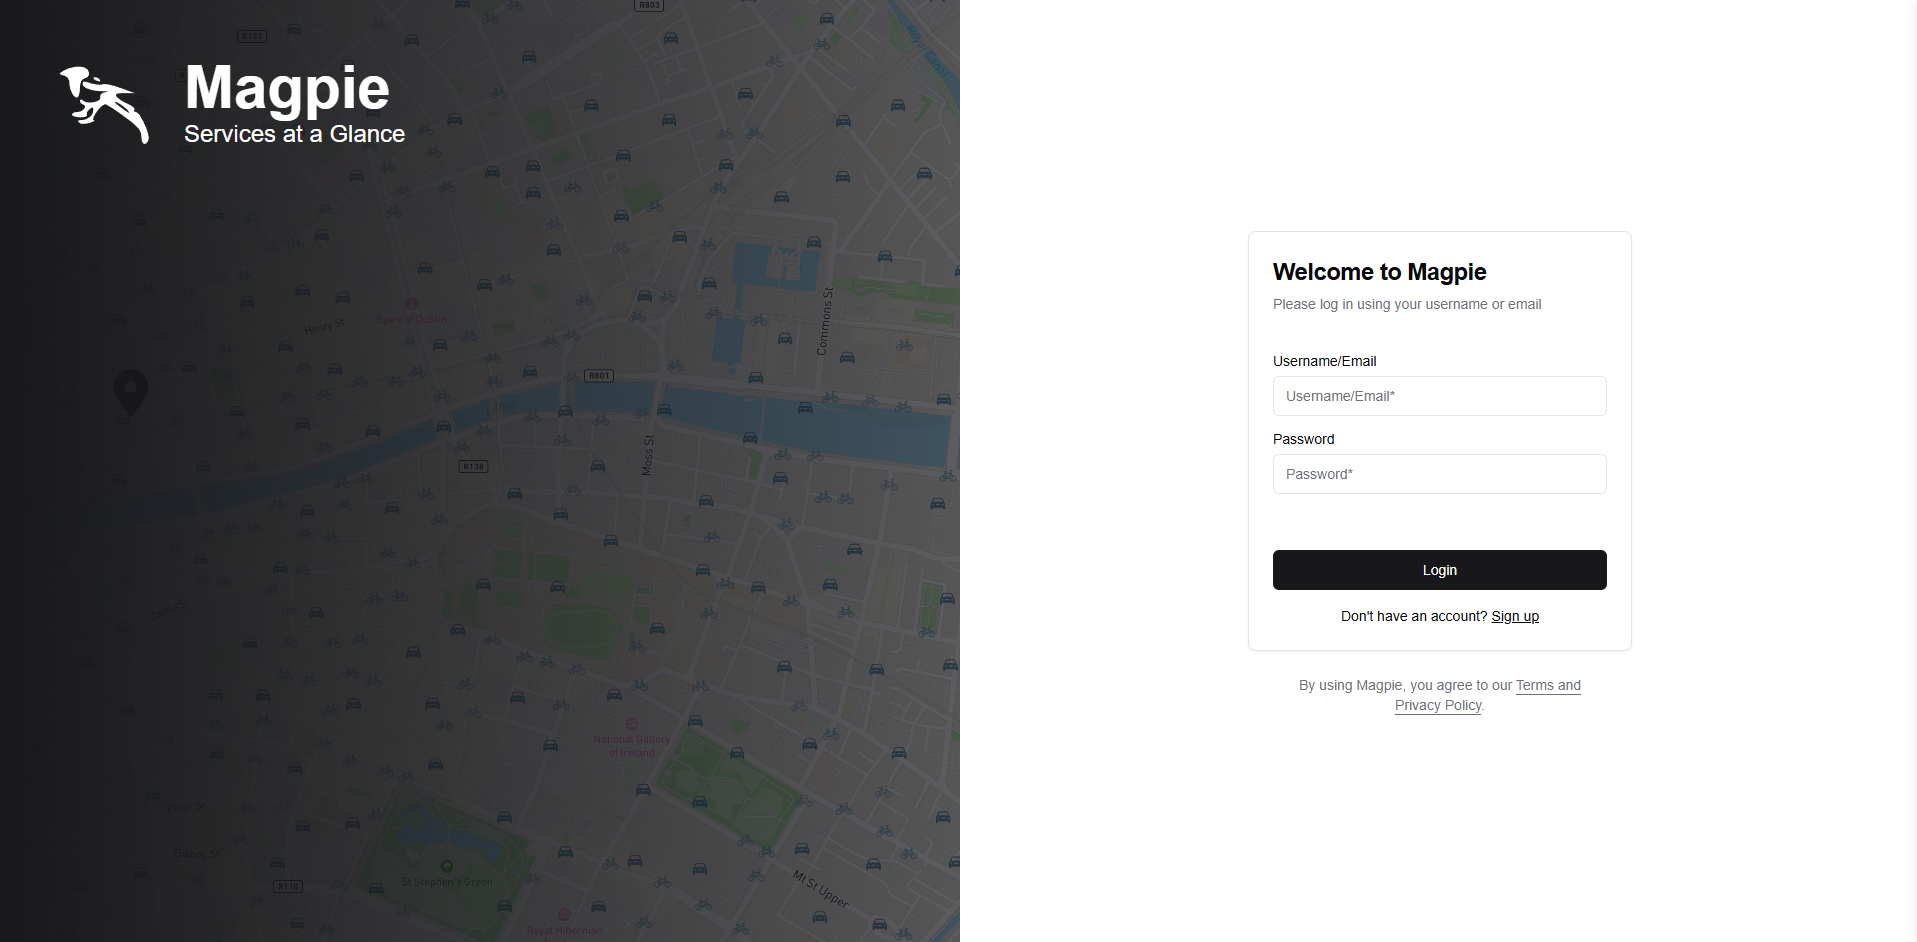
\includegraphics[width=1\textwidth]{images/site/login/login_page.png}
    \caption{The Login Page}
\end{figure}

The \textbf{Login} page is designed to provide a smooth and efficient experience for registered users to access their Magpie accounts. This page ensures that returning users can log in quickly and securely, reinforcing the brand’s focus on user experience and data protection.

\textbf{Header section}

The header section plays a crucial role in maintaining consistent branding.0
\begin{itemize}
    \item{} \textbf{Magpie Logo:} Just like on the signup page, the \textbf{Magpie logo} is prominently displayed at the top of the page. The logo serves to create immediate brand recognition and assures users they are on the official platform. It is positioned alongside the tagline \textbf{`Services at a Glance'}, which reinforces the site's purpose—providing users with an easy and visual way to view available public services across Dublin.
    \item{} \textbf{Visual Consistency:} The design maintains visual consistency with the rest of the platform, using the same color schemes and font styles, ensuring that users immediately feel familiar with the interface. This consistency across pages helps enhance the overall user experience and navigational ease. 
\end{itemize}

\textbf{Form Inputs}

The core functionality of the page revolves around the \textbf{login form}, which requires users to enter their credentials to access their accounts.

\begin{itemize}
    \item{} \textbf{Username Input:} The form begins with an input field for the \textbf{Username}. This field is critical for user identification, allowing the platform to locate the correct account. The label for the input field is clearly marked, and the field is large enough for easy typing, which is particularly important for mobile users.
    \item{} \textbf{Password Input:} Below the username, users are required to enter their \textbf{Password}. This ensures secure access to the platform and protects user data. The password input field features a `Show' button, allowing users to toggle between obscured and visible text, which reduces errors during login, especially when using complex passwords. This feature enhances user convenience, making it easier for them to confirm they are entering the correct password.
\end{itemize}

\newpage{}

\paragraph{Homepage}\mbox{}

\begin{figure}[h]
    \centering{}
    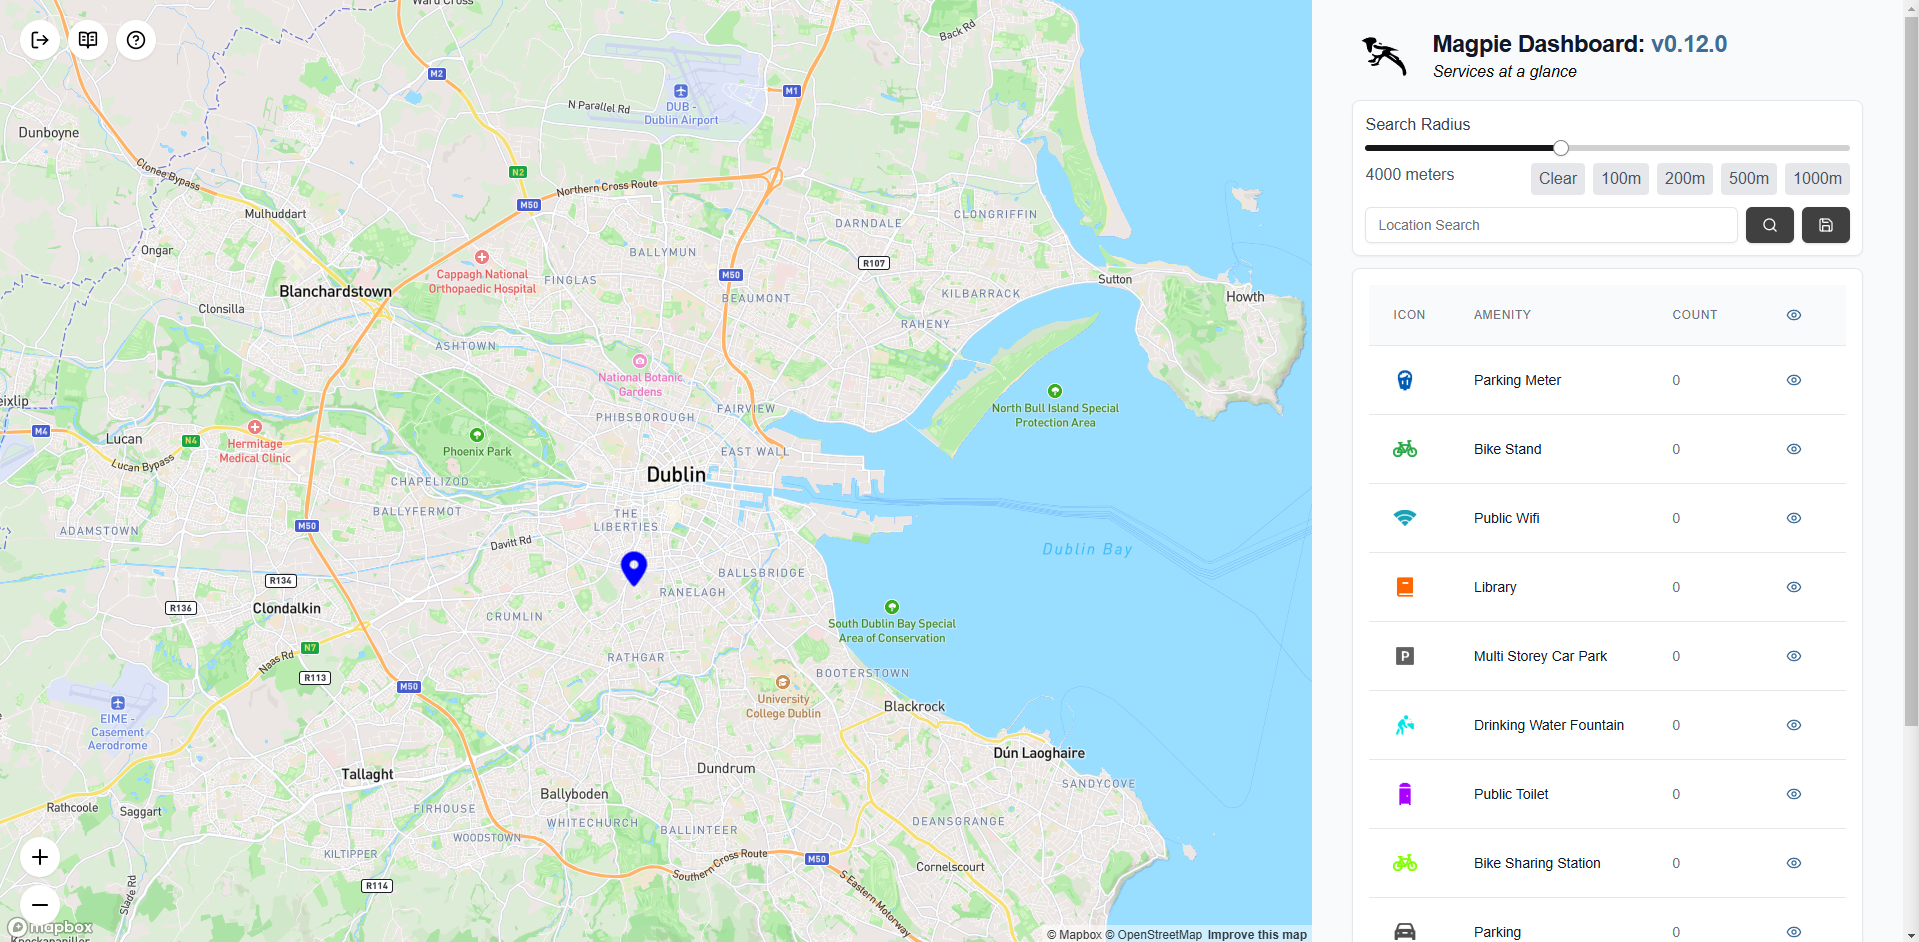
\includegraphics[width=1\textwidth]{images/site/home/homepage_1.png}
    \caption{Homepage}
\end{figure}




\textbf{Introduction}

Upon landing on the page, users are greeted with a map interface centred on Dublin and its surroundings, displaying various public services available in the area. The page provides an interactive map to explore amenities and services in the region, such as parking meters, bike stands, public Wi{-}Fi, libraries, and more.

\textbf{Top section}

\begin{itemize}
    \item{} \textbf{Logo and Title:} At the top{-}right corner, you’ll see the Magpie logo and the dashboard title.
    \item{} \textbf{Search Bar and Radius Control:} Beneath the header, there is a search bar to find specific locations, accompanied by a `Search Radius' slider. This allows users to set the distance range for viewing available services. The slider can adjust the search radius between 1m and 10km.
\end{itemize}

\textbf{Map interface}

The main focus of the page is the map, which occupies a large portion of the screen

\begin{itemize}
    \item{} \textbf{Interactive Map:} The map is interactive, powered by Mapbox, where users can zoom in and out using a mouse or touchpad gestures (pinch to zoom). Location markers represent different public services, such as parking meters or bike stands. These markers provide both a visual and interactive experience for users.
    \item{} \textbf{Service Markers:} Clicking on any marker will display detailed information about the selected service, such as its name, type, and available count.
\end{itemize}

\textbf{Sidebar}

\begin{itemize}
    \item{} \textbf{Interactive Map:} The map is interactive, powered by Mapbox, where users can zoom in and out using a mouse or touchpad gestures (pinch to zoom). Location markers represent different public services, such as parking meters or bike stands. These markers provide both a visual and interactive experience for users.
    \item{} \textbf{Service Markers:} Clicking on any marker will display detailed information about the selected service, such as its name, type, and available count.
\end{itemize}

\textbf{Onboarding Tour:}

A guided onboarding process walks the user through the various features of the platform, highlighting key elements such as:

\begin{enumerate}
    \item{} \textbf{Search Radius:} Adjusting the search range.
    \item{} \textbf{Marker Data:} Information displayed upon selecting a service marker.
    \item{} \textbf{Selecting Amenities:} The ability to toggle amenity visibility.
    \item{} \textbf{Map Interaction:} How  to click and zoom on the map to select locations.
\end{enumerate}

\textbf{Footer and Cookie Consent:}

\textbf{Footer:} At the bottom of the page, the user is shown a cookie consent banner, offering the option to accept or decline cookies for the site’s functionality.

This page is designed to provide users with an easy{-}to{-}use and interactive interface to view and search for public services across Dublin. The combination of a detailed map with customizable filters and an intuitive onboarding process ensures that users can quickly understand and make use of the platform’s features. The inclusion of interactive elements like the service markers and radius control further enhances the user experience.


\paragraph{History Page}\mbox{}

The \textbf{History} page in Magpie provides users with a clear view of their saved location data, allowing them to easily manage and track their previously stored points of interest related to public services. This page is designed to help users interact with their historical data in a seamless and intuitive way.

\textbf{Header Section}
\begin{itemize}
    \item{} \textbf{Navigation Back Button:} Located at the top left of the page, there is a prominent \textbf{Back Button}. This button allows users to quickly navigate back to the previous page. It’s styled with an icon of a leftward arrow, making it easily identifiable. Its positioning ensures that users can always return to the previous screen without confusion.
    \item{} \textbf{Page Title and Description:} The main section of the header includes a title \textbf{`Saved Locations'} displayed in a large, bold font. This title makes it clear to the user that they are viewing a list of locations they have saved. Beneath the title, a brief description—\textbf{`Here's a list of your saved amenity locations!'}—adds context to the page, helping users understand the purpose of the section.
\end{itemize}